% This file is part of the stream_information project.
% Copyright 2017 the authors. All rights reserved.

% # style notes
% - it is Cram\'er--Rao not Cram\'er-Rao. And yet Fisher-matrix not Fisher--matrix.

% TODO:
% - Reference for the dustmaps package? See software section.

\documentclass[modern]{aastex62}

\usepackage{amsmath}

% typography
\setlength{\parindent}{1.\baselineskip}
\newcommand{\acronym}[1]{{\small{#1}}}
\newcommand{\package}[1]{\textsl{#1}}
\newcommand{\gaia}{\textsl{Gaia}}
\newcommand{\pans}{\textsl{PanSTARRS}}
\newcommand{\DR}{\acronym{DR2}}
\newcommand{\msun}{\rm M_\odot}

% aastex parameters
% \received{not yet; THIS IS A DRAFT}
%\revised{not yet}
%\accepted{not yet}
% % Adds "Submitted to " the arguement.
% \submitjournal{ApJ}
\shorttitle{GD-1 in Gaia DR2}
\shortauthors{price-whelan \& bonaca}

%@arxiver{}

\begin{document}\sloppy\sloppypar\raggedbottom\frenchspacing % trust me

\title{Gaia DR2 view of the GD-1 stellar stream}

\author[0000-0003-0872-7098]{Adrian~M.~Price-Whelan}
\affiliation{Department of Astrophysical Sciences,
             Princeton University, Princeton, NJ 08544, USA}
\email{adrn@astro.princeton.edu}
\correspondingauthor{Adrian M. Price-Whelan}

\author[0000-0002-7846-9787]{Ana Bonaca}
\affil{Harvard--Smithsonian Center for Astrophysics, Cambridge, MA 02138, USA}


\begin{abstract}\noindent % trust me
Tidally-disrupted globular clusters are transformed into thin, dynamically-cold streams
of stars that are extremely valuable tracers of the large- and small-scale
distribution of matter in the Galaxy.
Most of such streams discovered in the Milky Way reside in its halo, and are therefore primarily sensitive to the distribution of dark matter.
We present a sample of highly-probable members of the longest cold stream, GD-1, selected on small parallaxes and retrograde proper motions provided by the \gaia\ mission, and \pans\ photometry consistent with an old and metal-poor population at a distance of $\sim10\,$kpc.
This selection extended the stream by $10^\circ$(?), revealed a possible location of the progenitor and mapped significant density variations along the stream in unprecedented detail.
In addition to several prominent gaps, for the first time we also find evidence of stream members off the main track.
No(?) secular formation mechanisms predict the existence of such spurs, but they are a natural result of a stream interaction with a massive perturber.
Based on the impulse approximation arguments, we estimate that the detected underdensity and the associated spur could have been induced by a perturbation of a $\sim10^7\,\rm M_\odot$(?) object $\sim 0.5\,$Gyr ago.
Our model of GD-1 indicates that the stream crosses the Galactic plane at a large radius, which puts the likely origin of the perturber beyond the stellar disk.
\end{abstract}

\keywords{Galaxy: halo --- dark matter}

\section{Introduction}
\label{sec:intro}

Dynamically cold stellar streams are formed from the tidal disruption of stellar
systems by the gravitational field of their host galaxy (e.g.,
\citealt{Johnston:1998}).
Over 30 candidate stellar streams have been discovered throughout the halo of
the Milky Way and have a wide range of properties such as length, velocity
dispersion, and density (e.g., \citealt{SoManyPeople,Bonaca:2012}; see also the
recent review \citealt{Grillmair:2006, Newberg:2016}).
Of the thin, likely globular-cluster-origin streams, only two have clear
progenitor systems: NGC 5466 (\citealt{TODO}) and Palomar 5 (\citealt{TODO}).

Stellar streams are

\citealt{Bonaca:2018}

Dynamical modeling of stellar streams or models of mean stream tracks have been used


Though it has been shown with many independent methods that modeling these thin streams can place strong constraints on the gravitational potential in which they form \citep{apw14,TODO}, many efforts to apply these models to real streams around the Milky Way have been hampered by the small number of known progenitor systems.


We revisit...do not try to model or fit for Galactic potential. Focus on stream properties, data.

\section{Data}
\label{sec:data}

- Transform to GD-1 coordinates (Koposov et al.)
    - Can see deviation from great circle
- Cut to be close to latitude = 0
- Cut to get proper motion over-density
- Color-magnitude filtering

Figure 1:
- PM cut (panel a)
- PM + CMD cut (panel b)
- SFD (panel c)??

Comment on these here - add figure for both in Appendix?
- Dust / no significant extinction - combine with other figure
- Scanning pattern - just discuss, no figure

Most of the clearly identifiable portions of the GD-1 stream are located at high
Galactic latitudes ($b > 35^\circ$), and we therefore do not expect significant
dust extinction or variations in extinction along the stream.
\figurename~\ref{fig:sfd} shows the $V$-band extinction in the region around the
GD-1 stream, computed from the Schlegel-Finkbeiner-Davis extinction map
(\cite{Schlegel:1998}; hereafter SFD).
Vertical lines indicate the two regions clearly identifiable as under-densities
from the proper-motion-selected stream members.
The maximum $A_V$ is $\approx$0.07 mag in both the under-density and gap
regions.
The dispersion in $A_V$ in the region $-60^\circ < \phi_1 < 0^\circ$ and
$-1^\circ < \phi_1 < 1^\circ$ is $\sigma_{A_V} \approx 0.03~\textrm{mag}$.

% Notebook: GD1-dust-and-completeness
\begin{figure}[h]
\begin{center}
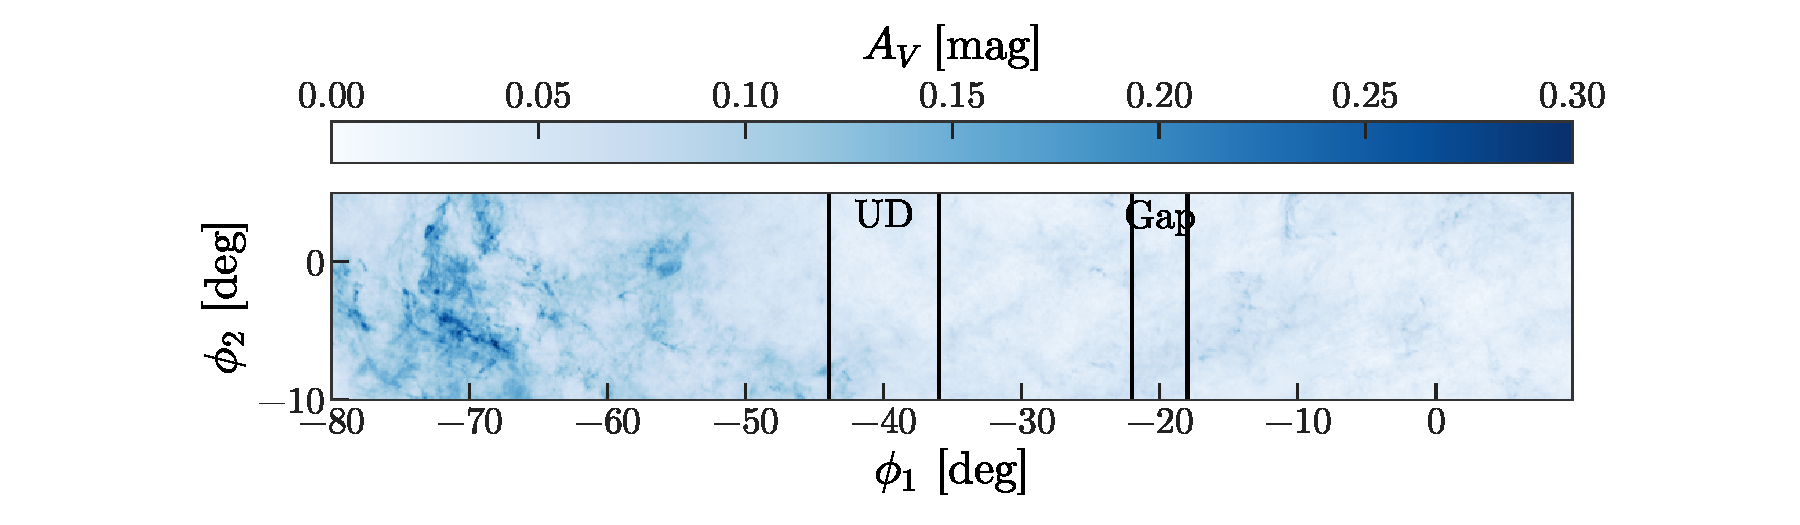
\includegraphics[width=\textwidth]{sfd.pdf}
\end{center}
\caption{%
Colored background shows the $V$-band extinction, $A_V$, in the GD-1
coordinate system.
Vertical lines roughly show the extents the identified under-density (UD) and
gap.
The maximum extinction in the UD or Gap regions is $\approx$0.07 mag.
\label{fig:sfd}
}
\end{figure}


\section{Results}
\label{sec:results}

\subsection{Global properties}
\label{sec:res_global}

\subsection{Gap}
\label{sec:res_gap}

\subsection{Underdensity}
\label{sec:res_underdensity}


\section{Discussion}
\label{sec:discussion}


\acknowledgements{
Gaia
Belokurov, Casey, Geha, Hogg, Johnston, Koposov, Lisanti, Schlafly, Spergel
This research was started at the NYC Gaia DR2 Workshop at the Center for Computational Astrophysics of the Flatiron Institute in 2018 April.
AB acknowledges generous support from the Institute for Theory and Computation at Harvard University.
All code used in this work and all results are available at \url{https://github.com/adrn/GD1-DR2}.
}

\software{
    \package{Astropy} \citep{astropy},
    \package{dustmaps}\footnote{\url{https://github.com/gregreen/dustmaps}},
    \package{gala} \citep{gala},
    \package{IPython} \citep{ipython},
    \package{matplotlib} \citep{mpl},
    \package{numpy} \citep{numpy},
    \package{scipy} \citep{scipy}
}

\bibliographystyle{aasjournal}
\bibliography{gd1}

\clearpage

\appendix
\section{Completeness check and data validation}
\label{sec:validate}

% % Notebook:
% \begin{figure}[h]
% \begin{center}
% \includegraphics[width=0.7\textwidth]{nvisits.pdf}
% \end{center}
% \caption{%
% TODO
% \label{fig:TODO}
% }
% \end{figure}


\end{document}
